\documentclass[journal]{IEEEtran}
\usepackage[a5paper, margin=10mm]{geometry}
%\usepackage{lmodern} % Ensure lmodern is loaded for pdflatex
\usepackage{tfrupee} % Include tfrupee package

%iffalse
\let\negmedspace\undefined
\let\negthickspace\undefined
\usepackage{gvv-book}
\usepackage{gvv}
\usepackage{cite}
\usepackage{amsmath,amssymb,amsfonts,amsthm}
\usepackage{algorithmic}
\usepackage{graphicx}
\usepackage{textcomp}
\usepackage{xcolor}
\usepackage{txfonts}
\usepackage{listings}
\usepackage{enumitem}
\usepackage{mathtools}
\usepackage{gensymb}
\usepackage{comment}
\usepackage[breaklinks=true]{hyperref}
\usepackage{tkz-euclide} 
\usepackage{listings}                                        
%\def\inputGnumericTable{}                                 
\usepackage[latin1]{inputenc}                                
\usepackage{color}                                            
\usepackage{array}                                            
\usepackage{longtable}                                       
\usepackage{calc}                                             
\usepackage{multirow}                                         
\usepackage{hhline}                                           
\usepackage{ifthen}                                           
\usepackage{lscape}
\usepackage{tabularx}
\usepackage{array}
\usepackage{float}
\usepackage{multicol}

\newcommand{\BEQA}{\begin{eqnarray}}
\newcommand{\EEQA}{\end{eqnarray}}
%\newcommand{\define}{\stackrel{\triangle}{=}}

\setlength{\headheight}{1cm} % Set the height of the header box
\setlength{\headsep}{0mm}     % Set the distance between the header box and the top of the text

%\usepackage[a5paper, top=10mm, bottom=10mm, left=10mm, right=10mm]{geometry}


\setlength{\intextsep}{10pt} % Space between text and floats

% Marks the beginning of the document
\begin{document}
\onecolumn
\bibliographystyle{IEEEtran}
\vspace{3cm}

%\renewcommand{\theequation}{\theenumi}
\numberwithin{equation}{section}
\numberwithin{figure}{section}
% \renewcommand{\thefigure}{\theenumi}
\renewcommand{\thetable}{\theenumi}

\title{Shortest Distance Between Curves}
\author{AI24BTECH11031 - Shivram S}
\maketitle

% \renewcommand{\thefigure}{\theenumi}
\renewcommand{\thetable}{\theenumi} 

\setcounter{section}{1}
\textbf{Question: } Find the shortest distance between the curves $x^2 + x + 12 = y$ and $x^2 + y^2 = 4$.
\bigskip

\textbf{Solution: } 

\begin{table}[h!]    
	\centering
	\begin{tabular}[12pt]{ |c| c| c|}
    \hline
    \textbf{Variable} & \textbf{Description} & \textbf{Value}\\
	\hline
	$C_1$ & Equation of first conic & $x^2 + x + 12 = y$\\
	\hline
	$C_2$ & Equation of second conic & $x^2 + y^2 = 4$\\
	\hline
\end{tabular}
	\caption{Variables Used}
\end{table}

We can rewrite the equations of the curves as
\begin{align}
    \vec{x}^\top\vec{V}_1\vec{x} + 2\vec{u}_1^\top\vec{x} + f_1 = 0 \\
    \vec{V}_1 = \myvec{1 & 0 \\ 0 & 0}, \vec{u}_1 = \myvec{\frac{1}{2} \\ -\frac{1}{2}}, f_1 = 12
\end{align}
and 
\begin{align}
    \vec{x}^\top\vec{V}_2\vec{x} + 2\vec{u}_2^\top\vec{x} + f_2 = 0 \\
    \vec{V}_2 = \myvec{1 & 0 \\ 0 & 1}, \vec{u}_2 = \myvec{0 \\ 0}, f_2 = -4
\end{align}

The shortest distance between the curves is along the common normal. Suppose the equation of the common
normal is
\begin{align}
    \vec{n}^\top\vec{x} = c
\end{align}

Suppose the line is normal to the second curve at the point $\vec{q}_2$.
The equation of the normal can be written as

\begin{align}
    \brak{\vec{V}_2\vec{q}_2 + \vec{u}_2}^\top\vec{R}\brak{\vec{x} - \vec{q}_2} = 0 \\
\end{align}
where $\vec{R} = \myvec{0 & 1 \\ -1 & 0}$ is the rotation matrix. Suppose $\vec{q}_2 = r\myvec{\cos\theta \\ \sin\theta}$.
We can rewrite the above equation as
\begin{align}
    \brak{\vec{V}_2\vec{q}_2 + \vec{u}_2}^\top\vec{R}\vec{x} &= \brak{\vec{V}_2\vec{q}_2 + \vec{u}_2}^\top\vec{R}\vec{q}_2  \\
    &= \brak{\myvec{1 & 0 \\ 0 & 1}\myvec{r\cos\theta \\ r\sin\theta} + \myvec{0 \\ 0}}\myvec{r\cos\theta \\ r\sin\theta} \\
    &= r^2\myvec{-\sin\theta \\ \cos\theta}^\top\myvec{\cos\theta \\ \sin\theta} = 0
\end{align}

Therefore $c = 0$ and the normal passes through the origin.

Suppose the line is normal to the first curve at the point $\vec{q}_1$.
The equation of the normal can be written as
\begin{align}
    \brak{\vec{V}_1\vec{q}_1 + \vec{u}_1}^\top\vec{R}\brak{\vec{x} - \vec{q}_1} = 0
\end{align}

Now, we can take $\vec{q}_1 = \myvec{q_x \\ q_y}$ to get
\begin{align}
    \brak{\vec{V}_1\vec{q}_1 + \vec{u}_1}^\top\vec{R}\vec{q}_1 = 0 \\
    \myvec{q_x + \frac{1}{2} \\ -\frac{1}{2}}^\top \myvec{0 & 1 \\ -1 & 0} \myvec{q_x \\ q_y} = 0 \\
    q_xq_y + \frac{1}{2}q_y + \frac{1}{2}q_x = 0 \label{eq1}
\end{align}

Now, since $\vec{q}_1$ lies on the first curve,
\begin{align}
    \myvec{q_x \\ q_y}^\top \myvec{1 & 0 \\ 0 & 0} \myvec{q_x \\ q_y} + 2\myvec{\frac{1}{2} \\ -\frac{1}{2}}^\top\myvec{q_x \\ q_y} + 12 = 0 \\
    q_y = q_x^2 + q_x + 12
\end{align} 
Substituting the value of $q_y$ in \ref{eq1} gives us
\begin{align}
   2q_x^3 + 3q_x^2 + 26q_x + 12 = 0 \\
\end{align}

Solving this equation gives us $q_x = -0.48$, which can be substituted in \ref{eq1}
to get $q_y = 11.75$. The other point of contact, $q_2$ is given by
$$
\vec{q}_2 = \frac{2}{\norm{\vec{q}_1}} \vec{q_1} = \myvec{-0.0816 \\ 1.998}
$$

Thus, the minimum distance between the curves is given by
\begin{align}
    \norm{\vec{q}_2 - \vec{q}_1} = 9.76
\end{align}

\begin{figure}
    \centering
    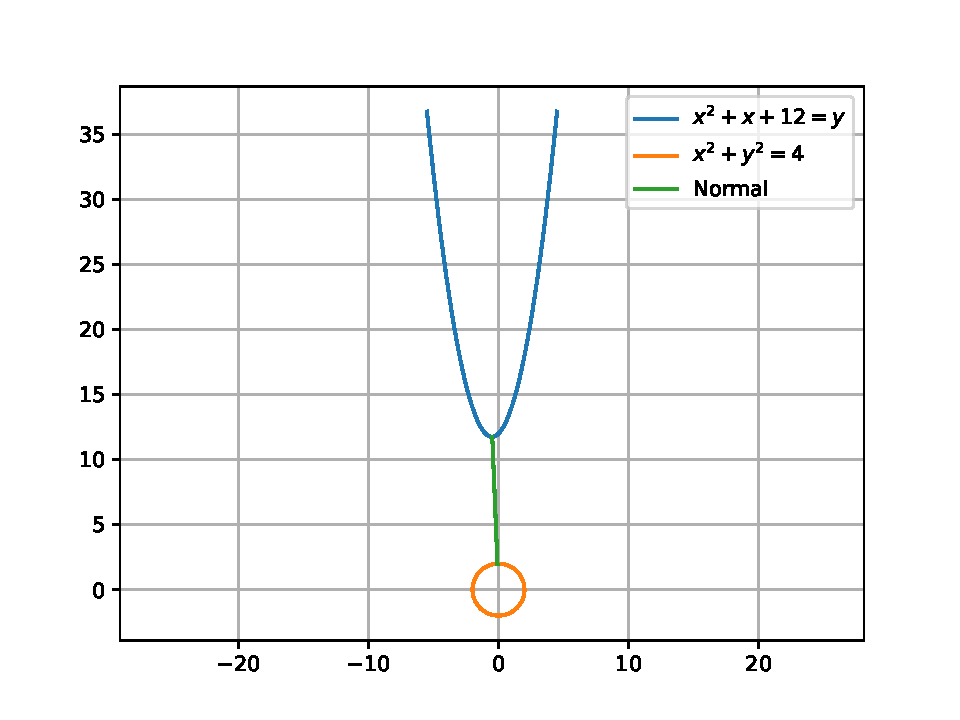
\includegraphics[width=0.7\linewidth]{figs/fig.pdf}
    \caption{The curves $x^2 + x + 12 = y$, $x^2 + y^2 = 4$, and their common normal.}
\end{figure}

\end{document}
